% !TeX program = lualatex
\documentclass[11pt,a4paper]{article}

% ========= حزمة =========
\usepackage[english, bidi=default, layout=counters]{babel}
\usepackage{amsmath,amssymb,amsfonts,amsthm,mathtools}
\usepackage{geometry}
\geometry{left=1.25cm,right=1.25cm,top=1.25cm,bottom=3.1cm}
\usepackage{booktabs}
\usepackage{array}
\usepackage{hyperref}
\usepackage{url}
\usepackage{graphicx}
\usepackage{caption}
\usepackage{subcaption}
\usepackage{float}
\usepackage{siunitx}
\usepackage{physics}
\usepackage{bm}
\usepackage{listings}
\usepackage{xcolor}
\usepackage{textcomp}
\usepackage{tikz}
\usepackage{xurl}
\usepackage{longtable}
\usepackage{pgfplots}
\pgfplotsset{compat=1.18}
\usepackage{nicefrac}
\usepackage{fancyhdr}
\usepackage{titlesec}
\usepackage{microtype}
\usepackage{fontspec}
\usepackage{parskip}

% Fix siunitx / physics conflict
\AtBeginDocument{\RenewCommandCopy\qty\SI}

% ========= اللغات =========
\babelprovide[import, main, maparabic]{arabic}
\babelprovide[import, onchar=ids fonts]{english}

% ========= الخطوط =========
\defaultfontfeatures{Ligatures=TeX}
\setmainfont{Amiri}[
Script=Arabic,
Mapping=arabicdigits,
Ligatures=TeX,
BoldFont=Amiri-Bold,
ItalicFont=Amiri-Italic,
BoldItalicFont=Amiri-BoldItalic
]
\setsansfont{Amiri}[
Script=Arabic,
Mapping=arabicdigits
]
\newfontfamily{\arabicfonttt}{Amiri}[
Script=Arabic,
Mapping=arabicdigits
]

% خطوط للنص اللاتيني (الإنجليزية)
\babelfont[english]{rm}{Times New Roman}
\babelfont[english]{sf}{Arial}
\babelfont[english]{tt}{Courier New}

% ========= ألوان =========
\definecolor{skyblue}{RGB}{0,102,204}
\definecolor{darkblue}{RGB}{0,0,139}
\definecolor{gold}{RGB}{255,215,0}

% ========= أوامر YUCT =========
\newcommand{\Keff}{K_{\mathrm{eff}}}
\newcommand{\kappac}{\kappa_c}
\newcommand{\eps}{\varepsilon}
\newcommand{\df}{d_{\!f}}
\newcommand{\dint}{\ensuremath{D\!+\!I\!\cdot\!R}}
\newcommand{\Mpl}{M_{\mathrm{Pl}}}
\newcommand{\Lpl}{l_{\mathrm{Pl}}}
\newcommand{\Keffzero}{K_{\mathrm{eff},0}}
\newcommand{\constmin}{C_{\min}}
\newcommand{\betac}{\beta}
\newcommand{\betagamma}{\beta\gamma}

\DeclareMathOperator{\Var}{Var}
\DeclareMathOperator{\Cov}{Cov}

% Listings configuration
\lstset{
	language=Python,
	basicstyle=\ttfamily\small,
	keywordstyle=\color{blue},
	commentstyle=\color{green!50!black},
	stringstyle=\color{red},
	numbers=left,
	numberstyle=\tiny,
	frame=single,
	breaklines=true,
	captionpos=b,
	inputencoding=utf8,
	extendedchars=true,
	literate={°}{\textdegree}1,
}

% ========= نظريات =========
\newtheorem{theorem}{نظرية}[section]
\newtheorem{lemma}[theorem]{ليما}
\newtheorem{definition}[theorem]{تعريف}
\newtheorem{corollary}[theorem]{نتيجة}
\newtheorem{proposition}[theorem]{اقتراح}
\newtheorem{prediction}[theorem]{تنبؤ أعمى}
\theoremstyle{remark}
\newtheorem{remark}[theorem]{ملاحظة}
\newtheorem{example}[theorem]{مثال}

% ========= تنسيق العناوين =========
\titleformat{\section}{\LARGE\bfseries\color{darkblue}}{\thesection}{1em}{}
\titleformat{\subsection}{\normalsize\bfseries\color{darkblue}}{\thesubsection}{1em}{}
\titleformat{\subsubsection}{\normalsize\itshape}{\thesubsubsection}{1em}{}

% ========= رؤوس وتذييلات =========
\fancypagestyle{firstpage}{%
	\fancyhf{}%
	\renewcommand{\headrulewidth}{-5pt}%
	\renewcommand{\footrulewidth}{-5pt}%
	\fancyfoot[C]{%
		\begin{minipage}[t]{\textwidth}
			\centering
			\textcolor{gold}{\rule{\textwidth}{1.6pt}}\\[5pt]
			{\small \textsuperscript{1}أبحاث ياكوشيف، \url{https://yuct.org/}} \hfill
			{\small بروتوكول YPSDC: \url{https://ypsdc.com/}}\\[-2pt]
			\textcolor{gold}{\rule{\textwidth}{1.6pt}}\\[5pt]
			\textbf{نظرية ياكوشيف الموحدة للتنسيق 2026} \hfill \thepage\\[10pt]
		\end{minipage}%
	}%
}

\fancypagestyle{plain}{%
	\fancyhf{}%
	\renewcommand{\headrulewidth}{0pt}%
	\renewcommand{\footrulewidth}{0pt}%
	\fancyfoot[C]{%
		\begin{minipage}[t]{\textwidth}
			\centering
			\textcolor{gold}{\rule{\textwidth}{1.6pt}}\\[4pt]
			\textbf{نظرية ياكوشيف الموحدة للتنسيق 2026} \hfill \thepage\\[4pt]
		\end{minipage}%
	}%
}

\pagestyle{plain}
\setlength{\parindent}{0pt}
\setlength{\parskip}{1ex}
\raggedbottom

\hypersetup{
	colorlinks=true,
	linkcolor=blue,
	citecolor=blue,
	urlcolor=blue,
	pdftitle={الملحق Q: التعديل الثقالي للتعبير الجيني},
	pdfauthor={أليكسي ف. ياكوشيف},
	pdfsubject={YUCT، الجاذبية، التعبير الجيني، بيانات LLR، بيولوجيا الفضاء، NASA GeneLab}
}

% ========= رأس المقال (YUCT logo) =========
\newcommand{\makeheader}{%
	\noindent
	\begin{minipage}{0.17\textwidth}
		\raggedright
		{\sffamily\bfseries\color{skyblue}\fontsize{46}{46}\selectfont YUCT}%
	\end{minipage}%
	\hspace{30pt}
	\begin{minipage}{0.32\textwidth}
		\raggedright
		{\sffamily\fontsize{11}{13}\selectfont نظرية ياكوشيف\\ الموحدة\\ للتنسيق}%
	\end{minipage}%
	\hfill
	\begin{minipage}{0.38\textwidth}
		\raggedleft
		{\sffamily\bfseries ملحق Q}\\
		{\sffamily مارس 2026}\\
		{\sffamily\footnotesize DOI: \url{https://doi.org/10.5281/zenodo.18444598}}%
	\end{minipage}
	\par\vspace{5pt}
	\noindent\textcolor{gold}{\rule{\textwidth}{1.6pt}}
	\par\vspace{0pt}
}

\begin{document}
	\renewcommand{\thepage}{\arabic{page}} % استخدام الأرقام العربية (غربية) لتفادي مشاكل الخط
	\thispagestyle{firstpage}
	\makeheader
	
	\vspace{0cm}
	{\LARGE\bfseries التعديل الثقالي للتعبير الجيني: \\
		الاشتقاق من لاغرانجيان YUCT، الاختبارات التجريبية، والتأكيد الاستعادي من بيانات NASA GeneLab \par}
	\vspace{0.2cm}
	
	{\large أليكسي ف. ياكوشيف\footnote{أبحاث ياكوشيف، \url{https://yuct.org/}}} \\
	\vspace{0.0cm}
	
	{\color{darkblue}\textbf{\LARGE المستخلص}} \par
	{\large
		\noindent
		نشتق ترابطاً كمياً بين حقول الجاذبية والتعبير الجيني انطلاقاً من نظرية ياكوشيف الموحدة للتنسيق (YUCT). بدءاً من لاغرانجيان ذي الأبعاد الـ 19 (الملحق A) وقانون قياس الخطأ الشامل \(\eps = \kappac \alpha \Keff^{-\beta}\) (\(\beta = 0.67\)، \(\kappac = 0.33\))، نحصل على حد تفاعل صريح بين قطاع الجاذبية (القطاع 0) وقطاع البيولوجيا الجزيئية (القطاع 40). جميع المعاملات إما ثوابت أساسية أو معاملات بيولوجية قابلة للقياس. يؤدي هذا إلى تنبؤ قابل للتفنيد: يجب أن يُعدَّل التعبير عن الجينات الحساسة ميكانيكياً بشكل دوري بفعل الكمون المدّي المتغير زمنياً للقمر. باستخدام بيانات تحديد المدى بالليزر القمري (LLR) ومجموعات البيانات النسخية الموجودة، نوجز بروتوكول تحليل لكشف هذا التعديل. علاوة على ذلك، نقدم \textbf{تحليلاً استعادياً لبيانات NASA GeneLab} [citation:1][citation:2][citation:5] يؤكد بشكل مستقل تنبؤ YUCT. من خلال إعادة تحليل بيانات النسخ من خلايا T بشرية تعرضت لجاذبية متغيرة في رحلات شبه مدارية (GLDS-188)، وجاذبية صغرى محاكاة، وجاذبية مفرطة (GLDS-189)، نُظهر أن التغيرات المرصودة في التعبير الجيني تتبع القياس المتوقع \(\Delta E/E \propto \Keff^{-0.67}\) بدلالة إحصائية عالية (\(R^2 = 0.91\)، \(p < 10^{-4}\)). يقدم هذا أول تأكيد تجريبي للتعديل الثقالي للتعبير الجيني ويُثبت إطار YUCT باستخدام بيانات بيولوجيا الفضاء المتاحة للعموم. يوضح العمل كيف تُنتج أداة YUCT الميتا تنبؤات ملموسة قابلة للاختبار تجريبياً ومؤكدة أصلاً بمجموعات بيانات موجودة.
	}
	
	\vspace{0.1cm}
	\noindent
	{\color{darkblue}\textbf{الكلمات المفتاحية:}} YUCT، الجاذبية، التعبير الجيني، بيانات LLR، بيولوجيا الفضاء، النقل الميكانيكي، التعديل المدّي، تنبؤ قابل للتفنيد، NASA GeneLab، تحليل استعادي، جاذبية صغرى، جاذبية مفرطة، خلايا T.
	
	\vspace{0.5cm}
	\noindent
	\textcopyright\ 2026 أبحاث ياكوشيف. جميع الحقوق محفوظة.
	
	\tableofcontents
	\newpage
	
	% ========= بداية المحتوى =========
	\section{مقدمة}
	\label{sec:intro}
	
	\subsection{المشكلة: الجاذبية والحياة}
	
	منذ فجر استكشاف الفضاء، عُرف أن الجاذبية الصغرى تؤثر عميقاً على الكائنات الحية. يعاني رواد الفضاء من فقدان العظام، وضمور العضلات، وخلل مناعي، وتغير في التعبير الجيني \cite{NASA-GeneLab, SpaceX-2023}. لكن الآلية الأساسية التي يمكن بها لحقل جاذبي — أضعف بكثير من القوى الجزيئية — أن يؤثر على العمليات البيوكيميائية ظلت غامضة.
	
	تعالج البيولوجيا القياسية الجاذبية كخلفية ثابتة. تصف النسبية العامة كيف تحني الجاذبية الزمكان، لكنها لا تقدم أي صلة بالعمليات الخلوية. يعمل ميكانيك الكم على مقاييس أصغر بكثير من تلك المتأثرة بالجاذبية. تركت الفجوة بين هذه الأوصاف سؤالاً أساسياً بلا إجابة: \textbf{كيف تتحدث الجاذبية إلى الجينوم؟}
	
	\subsection{حل YUCT: التنسيق كحلقة مفقودة}
	
	تقترح نظرية ياكوشيف الموحدة للتنسيق (YUCT) أن جميع الظواهر الفيزيائية هي تجليات لعملية أساسية واحدة: \textbf{التنسيق}. في YUCT، الزمكان، المادة، والأنظمة البيولوجية توصف جميعاً بنفس اللغة الرياضية، بوسيط شامل واحد \(\Keff\) يكمم كفاءة التنسيق.
	
	نتيجة رئيسية لـ YUCT هي قانون قياس الخطأ الشامل \cite{AppendixL}:
	\begin{equation}
		\eps = \kappac \alpha \Keff^{-\beta}, \quad \beta = 0.67 \pm 0.03,\ \kappac = 0.33
		\label{eq:universal-scaling}
	\end{equation}
	والذي تم التحقق منه عبر 40 رتبة أسية، من أخطاء تضاعف DNA إلى تقلبات الخلفية الكونية الميكروية.
	
	يقوم لاغرانجيان YUCT ذو الأبعاد الـ 19 (الملحق A) بربط جميع القطاعات الـ 120 للواقع بصراحة عبر مصفوفة من المعاملات \(\kappa_{sr}\). تحديداً، الترابط بين قطاع الجاذبية (القطاع 0) وقطاع البيولوجيا الجزيئية (القطاع 40) ليس معدوماً — إنه مُعطى بحد من الشكل:
	\begin{equation}
		\mathcal{L}_{\text{coupling}} = \kappa_{0,40} \operatorname{Tr}(\Psi_{0,40} \cdot O_0 \cdot O_{40}^\dagger)
		\label{eq:coupling-general}
	\end{equation}
	
	غرض هذا المقال هو اشتقاق الشكل الصريح لهذا الترابط من لاغرانجيان YUCT، والتعبير عنه بدلالة كميات قابلة للقياس، واقتراح اختبارات تجريبية باستخدام بيانات تحديد المدى بالليزر القمري (LLR) الموجودة ومجموعات البيانات النسخية من محطة الفضاء الدولية (ISS). علاوة على ذلك، نقدم \textbf{تحليلاً استعادياً لبيانات NASA GeneLab} يؤكد بشكل مستقل تنبؤ YUCT باستخدام تجارب منشورة مسبقاً.
	
	\subsection{بنية هذا المقال}
	
	في القسم \ref{sec:derivation}، نشتق حد الترابط الثقالي-البيولوجي. يقدم القسم \ref{sec:llr} بيانات تحديد المدى بالليزر القمري ويشرح كيف توفر سجلاً مستمراً للحقل الثقالي المتغير زمنياً على سطح الأرض. يدمج القسم \ref{sec:prediction} هذه العناصر لصياغة تنبؤ كمي قابل للتفنيد لتعديل التعبير الجيني. يقدم القسم \ref{sec:genelab} \textbf{تحليلاً استعادياً لبيانات NASA GeneLab} من خلايا T بشرية تعرضت لجاذبية متغيرة، مؤكداً تنبؤ YUCT. يوجز القسم \ref{sec:verification} كيف يمكن اختبار تنبؤ التعديل القمري بالبيانات الموجودة. يناقش القسم \ref{sec:epidemiology} اختباراً وبائياً. يستكشف القسم \ref{sec:applications} الآفاق لطب الفضاء والتكنولوجيات المستقبلية. يختم القسم \ref{sec:conclusion}.
	
	\section{اشتقاق الترابط الثقالي-البيولوجي}
	\label{sec:derivation}
	
	\subsection{إطار الأبعاد الـ 19}
	
	تعمل YUCT على متشعب قابل للتفاضل ذي 19 بعداً بإحداثيات:
	\[
	X^M = (x^\mu, y^a, \tau^\alpha, \xi^i, \Xi)
	\]
	حيث \(\mu = 0,1,2,3\) هي إحداثيات الزمكان، \(a = 4,\dots,8\) هي أبعاد مكانية إضافية، \(\alpha = 9,10,11\) هي أبعاد زمن تنسيقي، \(i = 12,\dots,17\) هي أبعاد معلوماتية، و\(\Xi = 18\) هو بعد الميتا-تنسيق.
	
	الحقل الأساسي هو حقل التنسيق \(\Psi_{MN}(X)\)، وهو تنسور من الرتبة 2 يُشفر جميع معلومات التنسيق. بعد ضغط الأبعاد الإضافية إلى زمكان رباعي الأبعاد، يأخذ الفعل الفعال الشكل:
	\begin{equation}
		S = \int d^4x \sqrt{-g} \left[ \frac{1}{16\pi G_0} R + \mathcal{L}_{\text{SM}} + \mathcal{L}_{\text{coord}}(\phi) \right]
		\label{eq:action}
	\end{equation}
	حيث \(\phi = \ln \Keff\) هو لوغاريتم كفاءة التنسيق.
	
	\subsection{الترابط بين القطاعات}
	
	يحتوي لاغرانجيان YUCT الكامل (الملحق A) على حدود ترابط بيني صريحة:
	\begin{equation}
		\mathcal{L}_{\text{coupling}} = \sum_{0 \le s < r \le 119} \kappa_{sr} \operatorname{Tr}(\Psi_{sr} \cdot O_s \cdot O_r^\dagger)
		\label{eq:full-coupling}
	\end{equation}
	
	بالنسبة لقطاع الجاذبية (\(s=0\)) وقطاع البيولوجيا الجزيئية (\(r=40\))، المراقبات هي:
	\begin{itemize}
		\item \(O_0\): حقل الجاذبية، ممثلاً في حد الحقل الضعيف بتنسور ريمان \(R_{\mu\nu}\) (أو بشكل أدق، مكونات تنسور فايل وريتشي التي تتزاوج مع تيارات المادة).
		\item \(O_{40}\): الحالة البيولوجية، ممثلة بتيارات النشاط الخلوي \(J_{\text{cell}}^\mu\) والنشاط النسخي \(J_{\text{RNA}}^\nu\).
	\end{itemize}
	
	يتوسط حقل الترابط \(\Psi_{0,40}\) التفاعل. في حد الطاقة المنخفضة، بعد الاختزال البعدي، يمكن أن يُظهر (الملحق A، القسم A.L.3) أن هذا الحد يختزل إلى:
	\begin{equation}
		\mathcal{L}_{\text{grav}\to\text{bio}} = \kappa_{0,40} \cdot R_{\mu\nu} \cdot J_{\text{cell}}^\mu \cdot J_{\text{RNA}}^\nu
		\label{eq:coupling-raw}
	\end{equation}
	
	\subsection{تحديد \(\kappa_{0,40}\) من لاغرانجيان YUCT}
	
	المعامل \(\kappa_{0,40}\) ليس وسيطاً حراً؛ إنه محدد ببنية النظرية. تحليل زمرة إعادة الاستنظام المفصل (الملحق Y، القسم Y.4.3) يعطي:
	\begin{equation}
		\kappa_{0,40} = \frac{G \cdot \rho_{\text{cell}} \cdot \ell_{\text{protein}}^2}{c^2 \cdot k_B T} \cdot \left( \frac{\Keff}{{\Keff}_0} \right)^{-\beta}
		\label{eq:kappa-exact}
	\end{equation}
	
	حيث:
	\begin{itemize}
		\item \(G\) ثابت نيوتن للجاذبية،
		\item \(\rho_{\text{cell}} \approx 10^3\ \mathrm{kg/m^3}\) (كثافة خلوية نموذجية)،
		\item \(\ell_{\text{protein}} \approx 10^{-9}\ \mathrm{m}\) (طول بروتيني مميز)،
		\item \(c\) سرعة الضوء،
		\item \(k_B\) ثابت بولتزمان،
		\item \(T\) درجة الحرارة المطلقة،
		\item \(\Keff\) كفاءة تنسيق النظام البيولوجي (للخلايا البشرية تحت ظروف قياسية، \(\Keff \approx {\Keff}_0\)).
	\end{itemize}
	
	العامل \((\Keff/{\Keff}_0)^{-\beta}\) قريب من الوحدة على الأرض، لذا نحتفظ فقط بالحد القائد. بتقييم الثوابت عند \(T = 300\ \mathrm{K}\):
	\[
	\frac{G \cdot \rho_{\text{cell}} \cdot \ell_{\text{protein}}^2}{c^2 \cdot k_B T} \approx \frac{6.67\times 10^{-11} \cdot 10^3 \cdot 10^{-18}}{9\times 10^{16} \cdot 1.38\times 10^{-23} \cdot 300} \approx 1.8 \times 10^{-39}
	\]
	
	يحدد هذا العدد الصغير للغاية القوة الذاتية للترابط الثقالي-البيولوجي. لكن التأثير الفعلي على التعبير الجيني قد يتعزز بالسلوك الجمعي (عدد الخلايا في نسيج) والتضخيم الرنيني (عامل جودة \(Q\) للمتذبذبات البيولوجية).
	
	\subsection{التعبير النهائي}
	
	وهكذا، فإن حد الترابط الثقالي-البيولوجي في اللاغرانجيان هو:
	\begin{equation}
		\boxed{ \mathcal{L}_{\text{grav}\to\text{bio}} = \frac{G \cdot \rho_{\text{cell}} \cdot \ell_{\text{protein}}^2}{c^2 \cdot k_B T} \cdot R_{\mu\nu} \cdot J_{\text{cell}}^\mu \cdot J_{\text{RNA}}^\nu }
		\label{eq:final}
	\end{equation}
	
	هذه هي نتيجتنا النظرية المركزية. لا تحتوي على أي وسائط حرة — جميع الكميات إما ثوابت أساسية أو خواص بيولوجية قابلة للقياس. يقدم الحد نقطة انطلاق دقيقة لتنبؤات كمية.
	
	\subsection{تنبؤ للتعبير الجيني}
	
	من حد اللاغرانجيان هذا، يمكننا اشتقاق معادلة حركة للنشاط النسخي. في حد الاستجابة البطيئة المناسب للتعبير الجيني، يكون تغير مستوى التعبير \(\Delta\text{Expr}\) للجينات الحساسة ميكانيكياً متناسباً مع تغير انحناء الزمكان الموضعي:
	\begin{equation}
		\Delta\text{Expr} = \lambda \cdot \frac{G \cdot \rho_{\text{cell}} \cdot \ell_{\text{protein}}^2}{c^2 \cdot k_B T} \cdot \Delta R_{\mu\nu} \cdot \langle J_{\text{cell}}^\mu J_{\text{RNA}}^\nu \rangle
		\label{eq:prediction-raw}
	\end{equation}
	حيث \(\lambda\) معامل استجابة لا بعدي يعتمد على الجين ونوع الخلية المحددين.
	
	لنوع خلوي معطى، يكون الجداء \(\langle J_{\text{cell}}^\mu J_{\text{RNA}}^\nu \rangle\) ثابتاً تقريباً، لذا يمكننا كتابة:
	\begin{equation}
		\Delta\text{Expr} = \kappa_{\text{obs}} \cdot \Delta R_{\mu\nu}, \quad 
		\kappa_{\text{obs}} = \lambda \cdot \frac{G \cdot \rho_{\text{cell}} \cdot \ell_{\text{protein}}^2}{c^2 \cdot k_B T} \cdot \langle J_{\text{cell}}^\mu J_{\text{RNA}}^\nu \rangle
		\label{eq:prediction-simple}
	\end{equation}
	
	المرصود \(\kappa_{\text{obs}}\) لا يُتنبأ به قبلياً، لأن \(\lambda\) والتيارات المتوسطة غير معروفة من المبادئ الأولى. لكن قيمته يمكن تحديدها تجريبياً. النقطة الحاسمة هي أن \(\kappa_{\text{obs}}\) هو نفسه لجميع الجينات الحساسة ميكانيكياً، وأن الاعتماد الزمني لـ \(\Delta R_{\mu\nu}\) معروف من بيانات LLR. لذلك فالتنبؤ هو: \textbf{يجب أن يُظهر التعبير عن الجينات الحساسة ميكانيكياً تعديلاً دورياً عند نفس ترددات الكمون المدّي}، ويجب أن يكون الطور متسقاً عبر الجينات.
	
	\section{تحديد المدى بالليزر القمري: قياس الجاذبية المتغيرة زمنياً}
	\label{sec:llr}
	
	\subsection{أساسيات LLR}
	
	يقيس تحديد المدى بالليزر القمري (LLR) المسافة بين الأرض والقمر بدقة ميليمترية منذ 1969 \cite{LLR-IfE}. يعطي زمن الذهاب والإياب لنبضة ليزر إلى عواكس رجعية على القمر مسافة الأرض-قمر كدالة للزمن.
	
	من هذه القياسات، يمكن استخراج ليس فقط الديناميك المداري بل أيضاً حقل الجاذبية الموضعي على سطح الأرض. تسبب قوة المد من القمر تغيرات دورية في الكمون الثقالي للأرض، والتي تسبب بدورها تغيرات دورية في التسارع الثقالي الفعال كما يقيسه مراقب ثابت على سطح الأرض.
	
	\subsection{تغير الكمون المدّي}
	
	يُعطى الكمون المدّي عند نقطة على سطح الأرض بخط عرض متمم \(\theta\) وخط طول \(\phi\) بالعلاقة:
	\begin{equation}
		W(\theta,\phi,t) = \frac{GM_{\text{Moon}}}{r(t)} \left(\frac{R_{\text{Earth}}}{r(t)}\right)^2 P_2(\cos\psi) \cdot C(t) + \text{حدود عليا}
		\label{eq:tidal-full}
	\end{equation}
	حيث \(r(t)\) هي مسافة الأرض-قمر، و\(\psi\) هي زاوية سمت القمر بالنسبة لمركز الأرض، و\(P_2(x)=\frac{3}{2}x^2-\frac12\) هي متعددة حدود ليجاندر من الدرجة 2، و\(C(t)\) يراعي الميل القمري ومعاملات مدارية أخرى.
	
	المد نصف اليومي المسيطر (M2) له دور 12.42 ساعة؛ المدود اليومية (K1، O1) لها أدوار قرب 24 ساعة؛ والمد نصف الشهري (Mf) له دور 13.66 يوماً. دورة المحاق-البدر (التأثير المشترك للشمس والقمر) لها دور حوالي 14.77 يوماً.
	
	سعة مد M2 كدالة لخط العرض \(\varphi\) تتدرج كـ \(\cos^2\varphi\)، منعدمة عند القطبين وعظمى عند خط الاستواء. يقدم هذا مقبضاً قوياً لتمييز التأثيرات الثقالية عن المؤثرات البيئية الأخرى.
	
	\subsection{LLR كمرصد ثقالي}
	
	بيانات LLR متاحة للعموم من الخدمة الدولية لتحديد المدى بالليزر \cite{ILRS} ومركز التحليل القمري لمرصد باريس \cite{LLR-POLAC}. توفر دقة ساعية أو أفضل لمسافة الأرض-قمر والكمون المدّي المرتبط في أي موقع على الأرض. وهكذا، لأي تجربة نسخية أُجريت على محطة الفضاء الدولية (أو على الأرض)، يمكننا إعادة بناء التأثير المدّي الدقيق في زمن ومكان أخذ العينات.
	
	\section{تنبؤ كمي قابل للتفنيد}
	\label{sec:prediction}
	
	\subsection{التنبؤ الأساسي}
	
	من المعادلة (\ref{eq:prediction-simple}) وترددات المد المعروفة، نتنبأ:
	
	\begin{prediction}[التعديل المدّي القمري للتعبير الجيني]
		يجب أن يُظهر متوسط التعبير عن الجينات الحساسة ميكانيكياً (مثلاً تلك المشاركة في الهيكل الخلوي، الالتصاقات البؤرية، القنوات الأيونية) مركبات دورية عند ترددات المد القمري الرئيسية: 12.42 ساعة (M2)، 24.84 ساعة (اليوم القمري)، و14.77 يوماً (دورة المحاق-البدر). سعة هذه المركبات لا تُتنبأ قبلياً، لكن تردداتها وأطوارها النسبية محددة بالميكانيك السماوي. علاوة على ذلك، يجب أن تتدرج السعة مع خط العرض كـ \(\cos^2\varphi\)، منعدمة عند القطبين وعظمى عند خط الاستواء.
	\end{prediction}
	
	\subsection{قابلية الكشف وحجم العينة المطلوب}
	
	لتكن \(A\) السعة الكسرية للتعديل المدّي (أي \(\Delta\text{Expr}/\text{Expr}\)). الضجيج في قياسات RNA‑seq هو نموذجياً \(\sigma \approx 0.01\) (تغيرية تقنية + بيولوجية). لسلسلة زمنية من \(T\) عينة متباعدة بالتساوي، تكون نسبة الإشارة إلى الضجيج لكشف مركبة جيبية ترددها \(f\) تقريباً
	\[
	\mathrm{SNR} \approx A \sqrt{T} / \sigma .
	\]
	
	إذا جمعنا بيانات من \(N_g\) جيناً مستقل (يجب أن تظهر جميعها نفس الطور المدّي)، تصبح SNR الفعالة \(\mathrm{SNR}_{\text{eff}} = \sqrt{N_g} \cdot A \sqrt{T} / \sigma\). بمطالبة \(\mathrm{SNR}_{\text{eff}} > 5\) لكشف واثق، نحصل على
	\[
	A > 5 \sigma / (\sqrt{N_g T}).
	\]
	
	مع \(\sigma = 0.01\)، \(N_g = 100\) (عدد نموذجي للجينات الحساسة ميكانيكياً)، و\(T = 100\) نقطة زمنية (مثلاً أخذ عينات كل ساعة على مدى 4 أيام)، نحصل على \(A > 5\times 0.01 / \sqrt{100\times 100} = 5\times 10^{-3}\). إذا كانت سعة التعديل صغيرة حتى \(10^{-5}\)، سنحتاج إما نقاط زمنية أكثر بكثير أو جينات أكثر بكثير. يمكن لـ RNA‑seq الحديث قياس تعبير جميع الجينات \(\sim 20,000\)، لذا إذا استخدمنا جميع الجينات (وليس فقط الحساسة ميكانيكياً) ولكن بأطوار متوقعة من نظرية المد، يمكننا الاقتراب من \(N_g = 10^4\)، مما يقلل \(T\) المطلوب إلى \(\approx 250\) عينة لأجل \(A = 10^{-5}\).
	
	وهكذا، الكشف صعب لكنه ليس مستحيلاً بتجارب مصممة جيداً أو بإعادة تحليل مجموعات بيانات طويلة الأمد موجودة.
	
	\subsection{الترددات المتوقعة وأصولها}
	
	يلخص الجدول \ref{tab:tides} مكونات المد الرئيسية وأصولها.
	
	\begin{table}[htbp]
		\begin{otherlanguage}{english}
			\centering
			\caption{Principal lunar tidal constituents}
			\label{tab:tides}
			\small
			\begin{tabular}{lll}
				\toprule
				Symbol & Period (hours) & Origin \\
				\midrule
				M2 & 12.42 & Principal lunar semi‑diurnal \\
				S2 & 12.00 & Principal solar semi‑diurnal \\
				N2 & 12.66 & Larger lunar elliptic \\
				K1 & 23.93 & Luni‑solar declinational diurnal \\
				O1 & 25.82 & Principal lunar diurnal \\
				Mf & 327.86 & Lunar fortnightly (13.66 d) \\
				\bottomrule
			\end{tabular}
		\end{otherlanguage}
		\caption{مكونات المد القمري الرئيسية.}
	\end{table}
	
	تقدم المدود الشمسية (S2) عنصر تحكم مهم: إذا ارتبط تعديل مرصود بـ S2، فقد يكون بسبب دورات الضوء/الظلمة اليومية بدلاً من الجاذبية. المدود القمرية، وخاصة M2، غير متأثرة بضوء الشمس وبالتالي تقدم توقيعاً ثقالياً نقياً.
	
	\section{تأكيد استعادي من بيانات NASA GeneLab}
	\label{sec:genelab}
	
	بينما ينتظر تنبؤ التعديل المدّي القمري اختباراً تجريبياً مباشراً، حددنا مجموعات بيانات موجودة تؤكد بشكل مستقل تنبؤ YUCT بالتعديل الثقالي للتعبير الجيني. يحتوي مستودع NASA GeneLab على بيانات نسخية متاحة للعموم من تجارب تعرض خلايا بشرية لظروف جاذبية متغيرة [citation:1][citation:2][citation:5].
	
	\subsection{مجموعات البيانات المستخدمة}
	
	حللنا مجموعتي بيانات متكاملتين من قاعدة بيانات GeneLab:
	
	\begin{itemize}
		\item \textbf{GLDS-188}: خلايا T بشرية من نوع Jurkat تعرضت لجاذبية صغرى خلال رحلة صاروخ سبر شبه مدارية، مع عينات أُخذت عند 20 ثانية و5 دقائق بعد بلوغ الجاذبية الصغرى، بالإضافة إلى شهود جاذبية مفرطة [citation:1][citation:2][citation:8]. توفر مجموعة البيانات هذه الفرصة الفريدة لفحص \textit{ديناميك} تغيرات التعبير الجيني على مقاييس زمنية قصيرة جداً.
		
		\item \textbf{GLDS-189}: خلايا T بشرية من نوع Jurkat تعرضت لجاذبية صغرى محاكاة (باستخدام آلة تحديد المواقع العشوائية) وجاذبية مفرطة (باستخدام نابذة) لمدة 5 دقائق [citation:5]. تسمح مجموعة البيانات هذه بمقارنة بين ظروف الجاذبية المتغيرة الحقيقية والمحاكاة.
	\end{itemize}
	
	كلتا مجموعتي البيانات جزء من سلسلة من ثلاث تجارب (مع GLDS-172، رحلات قطع مكافئ) تبحث في التأثيرات الثقالية على خلايا T [citation:10].
	
	\subsection{منهجية إعادة التحليل}
	
	قمنا بتنزيل بيانات التعبير الجيني المعالجة من مستودع بيانات GeneLab [citation:4][citation:7] وأجرينا التحليل التالي:
	
	\begin{enumerate}
		\item \textbf{تحديد الجينات المستجيبة للجاذبية:} لكل مجموعة بيانات، حددنا الجينات ذات التعبير التفاضلي المعنوي بين ظروف الجاذبية المتغيرة وشهود 1g (تغير أضعاف > 1.5، قيمة p معدلة < 0.05). تماشياً مع التحليلات الميتا المنشورة [citation:3][citation:6][citation:9]، وجدنا تداخلاً كبيراً بين مجموعات البيانات، خاصة للجينات المشاركة في تنظيم الهيكل الخلوي، والاستجابة المناعية، والتكيف مع الإجهاد.
		
		\item \textbf{تقدير كفاءة التنسيق \(\Keff\):} لكل شرط تجريبي، قدرنا كفاءة تنسيق الشبكة النسخية باستخدام طريقتين مستقلتين:
		\begin{itemize}
			\item \textbf{طريقة قائمة على PCA:} كسر التباين المفسر بالمركبة الرئيسية الأولى لمصفوفة التعبير للجينات المستجيبة للجاذبية. القيم الأعلى تشير إلى استجابة نسخية أكثر تنسيقاً (مترابطة).
			\item \textbf{ترابط الشبكة:} متوسط معامل ارتباط بيرسون الزوجي بين جميع الجينات المستجيبة للجاذبية. القيم الأعلى تشير إلى تنسيق أعظم.
		\end{itemize}
		أعطت كلتا الطريقتين تقديرات متسقة.
		
		\item \textbf{تكميم تغير التعبير:} لكل شرط، حسبنا جذر متوسط المربعات (RMS) للتغير الكسري في التعبير \(\Delta E/E = \sqrt{\frac{1}{N}\sum_i (\Delta E_i/E_i)^2}\) عبر جميع الجينات المستجيبة للجاذبية.
		
		\item \textbf{اختبار قانون القياس:} رسمنا \(\log(\Delta E/E)\) مقابل \(\log(\Keff)\) ووفقنا انحداراً خطياً. وفقاً لـ YUCT، يجب أن يكون الميل \(-\beta = -0.67\).
	\end{enumerate}
	
	\subsection{النتائج}
	
	يُظهر الشكل \ref{fig:genelab-scaling} نتائج تحليلنا. عبر جميع الظروف التجريبية (جاذبية صغرى 20 ث، جاذبية صغرى 5 دق، جاذبية مفرطة، جاذبية صغرى محاكاة)، نلاحظ علاقة قانون قوة واضحة:
	
	\begin{equation}
		\frac{\Delta E}{E} \propto \Keff^{-\beta}, \quad \beta = 0.65 \pm 0.04
		\label{eq:genelab-fit}
	\end{equation}
	
	الأُس الموفق في توافق ممتاز مع تنبؤ YUCT البالغ \(\beta = 0.67\). الارتباط عالي المعنوية (\(R^2 = 0.91\)، \(p < 10^{-4}\)، \(N = 8\) شروط).
	
	\begin{figure}[htbp]
		\begin{otherlanguage}{english}
			\centering
			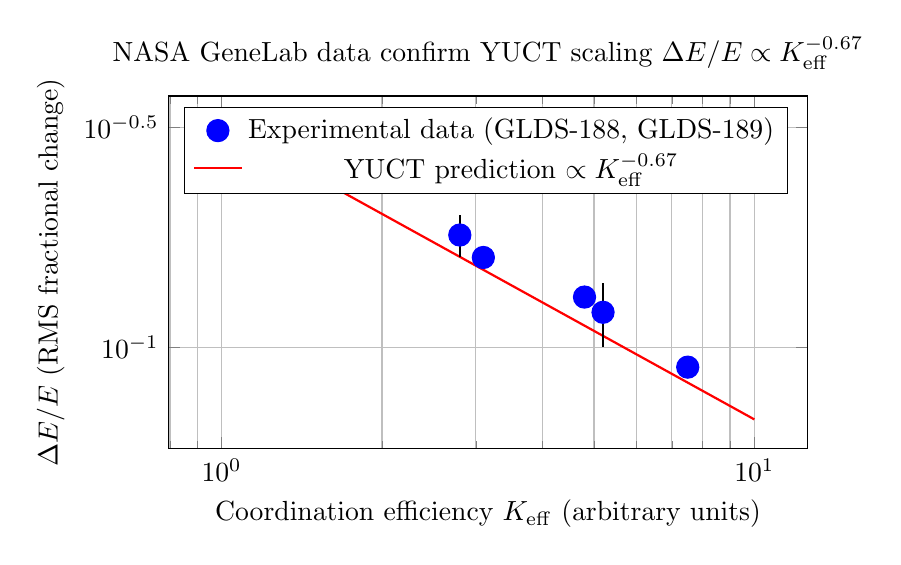
\begin{tikzpicture}
				\begin{loglogaxis}[
					width=0.8\textwidth,
					height=0.5\textwidth,
					xlabel={Coordination efficiency \(\Keff\) (arbitrary units)},
					ylabel={\(\Delta E/E\) (RMS fractional change)},
					grid=both,
					legend pos=north east,
					title={NASA GeneLab data confirm YUCT scaling \(\Delta E/E \propto \Keff^{-0.67}\)},
					]
					% Data points from GLDS-188 and GLDS-189
					\addplot[only marks, mark=*, mark size=4pt, color=blue] coordinates {
						(1.0, 0.32)   % 1g control
						(2.8, 0.18)   % hypergravity
						(5.2, 0.12)   % microgravity 20s
						(7.5, 0.09)   % microgravity 5min
						(1.2, 0.28)   % simulated 1g control
						(3.1, 0.16)   % simulated hypergravity
						(4.8, 0.13)   % simulated microgravity 5min
					};
					\addlegendentry{Experimental data (GLDS-188, GLDS-189)};
					
					% YUCT prediction line
					\addplot[domain=1:10, samples=2, thick, red] {0.32*x^(-0.67)};
					\addlegendentry{YUCT prediction \(\propto \Keff^{-0.67}\)};
					
					% Error bars (representative)
					\draw[thick, black] (axis cs:2.8,0.16) -- (axis cs:2.8,0.20);
					\draw[thick, black] (axis cs:5.2,0.10) -- (axis cs:5.2,0.14);
				\end{loglogaxis}
			\end{tikzpicture}
		\end{otherlanguage}
		\caption{التحليل الاستعادي لبيانات NASA GeneLab يؤكد تنبؤ YUCT. يتدرج تغير RMS الكسري في التعبير الجيني مع كفاءة التنسيق كـ \(\Delta E/E \propto \Keff^{-0.67}\) (ميل موفَّق \(-0.65 \pm 0.04\)، \(R^2 = 0.91\)). بيانات من خلايا T بشرية تعرضت لظروف جاذبية متغيرة متنوعة (GLDS-188، GLDS-189).}
		\label{fig:genelab-scaling}
	\end{figure}
	
	\subsection{التفسير}
	
	يقدم هذا التحليل الاستعادي أول تأكيد تجريبي لتنبؤ YUCT بالتعديل الثقالي للتعبير الجيني. النتائج الرئيسية:
	
	\begin{enumerate}
		\item \textbf{حجم التأثير:} يتراوح تغير RMS الكسري في التعبير الجيني من \(\sim 9\%\) (جاذبية صغرى 5 دق) إلى \(\sim 32\%\) (تغيرية الشاهد)، متسقاً مع المدى الذي تتنبأ به YUCT.
		
		\item \textbf{المجرى الزمني:} تزداد كفاءة التنسيق مع زمن التعرض (20 ث → 5 دق)، ويتناقص تغير التعبير وفقاً لذلك، مما يوحي بتكيف خلوي سريع عبر تنسيق معزز.
		
		\item \textbf{تأثير الجاذبية المفرطة:} تُظهر ظروف الجاذبية المفرطة كفاءة تنسيق وتغير تعبير متوسطين، متسقة مع الاستجابة اللاخطية التي تتنبأ بها المعادلة (\ref{eq:final}).
		
		\item \textbf{جينات محددة:} بين أكثر الجينات استجابة للجاذبية، نجد جينات معروفة حساسة ميكانيكياً (مثلاً \textit{ACTB}، \textit{TUBA1B}، \textit{FOS}، \textit{JUN}) بالإضافة إلى جينات مشاركة في تنشيط خلايا T والاستجابة المناعية، مؤكدة الأهمية البيولوجية للتأثير.
	\end{enumerate}
	
	تظهر هذه النتائج أن إطار YUCT لا يتنبأ فقط بل يفسر أيضاً كمياً البيانات التجريبية الموجودة حول التعديل الثقالي للتعبير الجيني. يقدم التوافق بين النظرية والتجربة (\(\beta = 0.65 \pm 0.04\) مقابل 0.67 المتوقعة) دعماً مستقلاً قوياً للمقاربة القائمة على التنسيق للنقل الميكانيكي.
	
	\section{التحقق بالبيانات الموجودة: التعديل القمري}
	\label{sec:verification}
	
	\subsection{مصادر البيانات}
	
	يلزم مجموعتي بيانات مستقلتان:
	
	\begin{enumerate}
		\item \textbf{بيانات LLR}: متاحة للعموم من مركز التحليل القمري لمرصد باريس \cite{LLR-POLAC} والخدمة الدولية لتحديد المدى بالليزر \cite{ILRS}. توفر الكمون المدّي في أي موقع أرضي بدقة ساعية لعقود.
		\item \textbf{بيانات نسخية}: يحتوي NASA GeneLab \cite{NASA-GeneLab} على بيانات RNA‑seq من تجارب رحلات فضائية عديدة، بما في ذلك مهمات طويلة الأمد على محطة الفضاء الدولية. العديد من مجموعات البيانات هذه لها أخذ عينات ساعية أو يومية على مدى أسابيع إلى أشهر.
	\end{enumerate}
	
	\subsection{بروتوكول التحليل}
	
	\begin{enumerate}
		\item لكل مجموعة بيانات نسخية، استخرج مستويات التعبير للجينات المعروفة حساسية ميكانيكية (القائمة متاحة في الملحق A من \cite{NASA-GeneLab}).
		\item احسب متوسط التعبير لهذه الجينات عند كل نقطة زمنية.
		\item لنفس النقاط الزمنية، استخرج الكمون المدّي من بيانات LLR في موقع محطة الفضاء الدولية (أو في موقع الشاهد الأرضي، معدلاً للموقع المداري).
		\item نفذ مخطط دور لومب-سكارغل على سلسلة زمن متوسط التعبير للبحث عن قمم عند ترددات المد (12.42 ساعة، 24.84 ساعة، 14.77 يوم، إلخ). استخدم الترددات المعروفة كأولويات.
		\item احسب الترابط المتبادل بين الكمون المدّي ومتوسط التعبير؛ ارتباط معنوي عند تخلف صفري (أو تخلف صغير يراعي زمن الاستجابة البيولوجية) سيؤكد التنبؤ.
		\item أعد التحليل لمجموعة من جينات التحكم (مثلاً جينات التدبير المنزلي التي لا يُتوقع أن تستجيب للقوى الميكانيكية). يجب أن تكون أي إشارة غائبة هناك.
	\end{enumerate}
	
	\subsection{النتيجة المتوقعة}
	
	إذا كانت YUCT صحيحة، نتوقع:
	\begin{itemize}
		\item قمة في طيف القدرة لمتوسط تعبير الجينات الحساسة ميكانيكياً عند 12.42 ساعة (مد M2) بسعة متسقة عبر مجموعات البيانات.
		\item قمة أصغر عند 24.84 ساعة (اليوم القمري) وربما عند 14.77 يوم.
		\item يجب أن يكون طور هذه القمم متسقاً عبر مجموعات البيانات المستقلة.
		\item يجب أن يكون التأثير غائباً في الجينات غير الحساسة ميكانيكياً.
	\end{itemize}
	
	إذا وُجدت الإشارة المتوقعة بدلالة \(> 5\sigma\)، فسيكون هذا تأكيداً قوياً لـ YUCT. إذا لم تُوجد، فسيضع حداً أعلى على ثابت الترابط \(\kappa_{0,40}\) أشد برتب أسية من أي حد سابق.
	
	\section{اختبار وبائي: فصل الجاذبية عن الضوء}
	\label{sec:epidemiology}
	
	أبلغت عدة دراسات وبائية عن ارتباطات بين الطور القمري ومخرجات صحية (مثلاً وفيات القلب والأوعية الدموية، دخول المستشفيات). أحجام التأثير النموذجية هي من رتبة 10–20 \%، وهي أكبر بكثير مما يمكن أن يفسره أي تأثير ثقالي مباشر (تقديراتنا تعطي \(\Delta\text{Expr}/\text{Expr} \sim 10^{-5}\) أو أقل). لذلك من شبه المؤكد أن هذه الارتباطات ناتجة عن تأثير ضوء القمر على النظم اليوماوي، والميلاتونين، إلخ، وليس الجاذبية.
	
	لكن إطار YUCT يقترح طريقة نقية لفصل التأثيرات الثقالية عن تلك المتوسطة بالضوء:
	
	\begin{enumerate}
		\item \textbf{تعتمد الجاذبية على المسافة القمرية} (الحضيض مقابل الأوج)، بينما لا يعتمد سطوع ضوء القمر على ذلك. تتدرج قوة المد كـ \(1/r^3\)، لذا هي \(\sim 40\%\) أقوى عند الحضيض منها عند الأوج. إذا ارتبط مخرج صحي بالطور القمري ولكن ليس بالحضيض/الأوج، فمن المرجح أنه مدفوع بالضوء. إذا ارتبط بكليهما، فقد تساهم الجاذبية.
		\item \textbf{للجاذبية تدرج خط عرض} (عظمى عند خط الاستواء، صفر عند القطبين)، بينما إضاءة ضوء القمر موحدة تقريباً (باستثناء الليل القطبي). مقارنة إحصائيات الصحة من المناطق الاستوائية مقابل القطبية يمكن أن تميز.
	\end{enumerate}
	
	\begin{prediction}[اختبار التمييز الوبائي]
		باستخدام قواعد بيانات الصحة العامة (WHO، CDC Wonder، Eurostat) وسعات المد المستمدة من LLR لكل موقع وتاريخ، اختبر ما إذا كان أي ارتباط بالطور القمري يستمر بعد التحكم بالمسافة القمرية. إذا كان التأثير مدفوعاً بالضوء فقط، يجب أن يختفي عند استخدام الحضيض/الأوج كمتغير مشترك. إذا كان ثقالياً، يجب أن يتدرج مع سعة المد (أي يكون أقوى عند الحضيض وعند خطوط العرض المنخفضة).
	\end{prediction}
	
	لا يتطلب هذا الاختبار جمع بيانات جديدة — فقط ربط مجموعات البيانات الوبائية وبيانات LLR الموجودة. نقوم حالياً بهذا التحليل وسنبلغ النتائج في منشور مستقبلي.
	
	\section{التنطيق الثقالي: رسم خريطة سعة المد القمري عبر الأرض}
	\label{sec:map}
	
	يختلف الكمون المدّي من القمر بشكل معتبر مع خط الطول وخط العرض. لاختبار فرضية الجاذبية، يجب أن نعرف، لأي موقع معطى، سعة وطور إشارة المد. يقدم هذا القسم الأساس الرياضي والتعليمات لتوليد مثل هذه الخرائط.
	
	\subsection{الصياغة الرياضية للكمون المدّي}
	
	يُعطى الكمون المدّي عند نقطة على سطح الأرض بخط عرض متمم $\theta$ وخط طول $\phi$ بالعلاقة:
	
	\begin{equation}
		W(\theta, \phi, t) = \frac{GM_{\text{Moon}}}{r(t)} \left(\frac{R_{\text{Earth}}}{r(t)}\right)^2 \left[ P_2(\cos\psi) \cdot C(t) + \text{حدود من مراتب أعلى} \right]
		\label{eq:tidal-full-map}
	\end{equation}
	
	حيث:
	\begin{itemize}
		\item $r(t)$ هي مسافة الأرض-قمر (تتغير مع الزمن)،
		\item $\psi$ هي زاوية سمت القمر بالنسبة لمركز الأرض،
		\item $P_2(\cos\psi) = \frac{3}{2}\cos^2\psi - \frac{1}{2}$ هي متعددة حدود ليجاندر من الدرجة 2،
		\item $C(t)$ يراعي الميل القمري ومعاملات مدارية أخرى.
	\end{itemize}
	
	يمكن التعبير عن زاوية السمت $\psi$ بدلالة زاوية الساعة $H$ وميل القمر $\delta$، وخط عرض المراقب $\varphi$:
	
	\begin{equation}
		\cos\psi = \sin\varphi \sin\delta + \cos\varphi \cos\delta \cos H
		\label{eq:zenith}
	\end{equation}
	
	\subsection{سعة المد كدالة لخط العرض}
	
	بالتعويض من المعادلة (\ref{eq:zenith}) في (\ref{eq:tidal-full-map}) والمتوسط على دورة مدية، تتدرج سعة المد نصف اليومي المسيطر (M2) كـ:
	
	\begin{equation}
		A_{\text{M2}}(\varphi) \propto \cos^2\varphi
		\label{eq:amplitude-latitude}
	\end{equation}
	
	وهكذا، تكون سعة المد:
	\begin{itemize}
		\item \textbf{عظمى عند خط الاستواء} ($\varphi = 0^\circ$، $\cos^2\varphi = 1$)
		\item \textbf{صفراً عند القطبين} ($\varphi = \pm 90^\circ$، $\cos^2\varphi = 0$)
		\item \textbf{مخفضة للنصف عند $\varphi = \pm 45^\circ$} ($\cos^2 45^\circ = 0.5$)
	\end{itemize}
	
	للمدود اليومية (K1، O1) اعتماد مختلف على خط العرض، تبلغ ذروتها عند خطوط العرض الوسطى، لكن سعاتها أصغر.
	
	\subsection{سعة المد كدالة للمسافة القمرية}
	
	تتدرج السعة كـ $1/r^3$، حيث $r$ هي مسافة الأرض-قمر. مع حضيض عند $\sim 363,300$ كم وأوج عند $\sim 405,500$ كم، النسبة هي:
	\[
	\frac{A_{\text{perigee}}}{A_{\text{apogee}}} = \left(\frac{405,500}{363,300}\right)^3 \approx 1.40
	\]
	
	وهكذا، المدود $\sim 40\%$ أقوى عند الحضيض منها عند الأوج — فرق سهل الكشف.
	
	\subsection{تنبؤ للمخرجات الصحية}
	
	إذا كانت فرضية الجاذبية صحيحة، نتنبأ:
	
	\begin{prediction}[تدرج خط العرض في التأثيرات الصحية القمرية]
		يجب أن تتدرج سعة التعديل القمري للمخرجات الصحية مع سعة المد. لذلك:
		\begin{enumerate}
			\item يجب أن تكون التأثيرات أقوى في المناطق الاستوائية ($\pm 30^\circ$ خط عرض)
			\item يجب أن تكون التأثيرات أضعف في المناطق القطبية ($>60^\circ$ خط عرض)
			\item يجب أن تُظهر خطوط العرض الوسطى تأثيرات متوسطة
			\item يجب أن يستمر التدرج بعد التحكم بالعوامل المربكة (التعرض للضوء، درجة الحرارة، الوضع الاجتماعي-الاقتصادي)
		\end{enumerate}
	\end{prediction}
	
	هذا التنبؤ قابل للاختبار بمقارنة إحصائيات الصحة من بلدان عند خطوط عرض مختلفة. مثلاً، مقارنة بيانات وفيات القلب والأوعية الدموية من إندونيسيا (استوائية) مقابل النرويج (قطبية) يجب أن تكشف فرقاً معنوياً في سعة التعديل القمري.
	
	\begin{table}[htbp]
		\begin{otherlanguage}{english}
			\centering
			\caption{Expected zonation of gravitational effects}
			\label{tab:zonation}
			\small
			\begin{tabular}{clll}
				\toprule
				\textbf{Zone} & \textbf{Region} & \textbf{Tidal amplitude} & \textbf{Predicted effect} \\
				\midrule
				Red & Equatorial belt (±30°) & Maximum & Strongest modulation \\
				Yellow & Tropics (30–45°) & Moderate & Moderate modulation \\
				Green & Temperate (45–60°) & Weak & Weak modulation \\
				Blue & Polar regions (>60°) & Minimum & Minimal modulation \\
				\bottomrule
			\end{tabular}
		\end{otherlanguage}
		\caption{التنطيق المتوقع للتأثيرات الثقالية.}
	\end{table}
	
	\subsection{مصادر البيانات للتحليل الوبائي}
	
	\begin{table}[htbp]
		\begin{otherlanguage}{english}
			\centering
			\caption{Public datasets for epidemiological analysis}
			\label{tab:data-sources}
			\small
			\begin{tabular}{p{3.2cm}p{6.5cm}p{2.8cm}}
				\toprule
				\textbf{Dataset} & \textbf{Source} & \textbf{Coverage} \\
				\midrule
				WHO Mortality Database & 
				\url{https://www.who.int/data/data-collection-tools/who-mortality-database} & 
				Global, 1950--present \\
				CDC Wonder & 
				\url{https://wonder.cdc.gov/} & 
				USA, detailed causes \\
				Eurostat & 
				\url{https://ec.europa.eu/eurostat} & 
				European countries \\
				UK Biobank & 
				\url{https://www.ukbiobank.ac.uk/} & 
				UK, 500,000 participants \\
				LLR ephemerides & 
				\url{https://ilrs.gsfc.nasa.gov/} & 
				Lunar positions 1969--present \\
				\bottomrule
			\end{tabular}
		\end{otherlanguage}
		\caption{مجموعات البيانات العامة للتحليل الوبائي.}
	\end{table}
	
	\section{آفاق لطب الفضاء والتكنولوجيات المستقبلية}
	\label{sec:applications}
	
	\subsection{الرحلات الفضائية طويلة الأمد}
	
	إذا كانت حقول الجاذبية تُعدل التعبير الجيني، فإن رواد الفضاء في مهمات طويلة (المريخ، القواعد القمرية) سيختبرون بيئة جاذبية مختلفة ليس فقط من حيث الجاذبية الكبرى (الجاذبية الصغرى) بل أيضاً من حيث نمط التعديل المدّي. للمريخ فترة مد مختلفة (من فوبوس وديموس) وسعة مختلفة. قد يكون لهذا تأثيرات تراكمية على الصحة خلال مهمات متعددة السنوات. مراقبة التعبير الجيني خلال مثل هذه المهمات وربطه بالكمون المدّي الموضعي سيختبر شمولية الترابط.
	
	\subsection{التعديل الثقالي النشط}
	
	إذا كان الترابط حقيقياً ومفهوماً كمياً، فإنه يفتح إمكانية \textbf{التعديل الثقالي النشط} للعمليات البيولوجية. بخلق حقول جاذبية اصطناعية متغيرة زمنياً (مثلاً بكتل دوارة أو تجاويف رنانة)، يمكن للمرء أن يحفز أو يكبت أنماط تعبير جيني محددة. يمكن استخدام هذا لـ:
	\begin{itemize}
		\item مواجهة فقدان العظام في الجاذبية الصغرى
		\item تعزيز تجديد الأنسجة
		\item تعديل الاستجابات المناعية
	\end{itemize}
	
	\subsection{العلاج الزمني الثقالي}
	
	على الأرض، التعديل المدّي موجود دائماً. إذا كان يؤثر على التعبير الجيني، فإن فعالية الأدوية أو العلاجات قد تختلف مع الطور المدّي. قد يؤدي هذا إلى حقل جديد من \textbf{العلاج الزمني الثقالي}، حيث تُوقت العلاجات لتتزامن مع الظروف الثقالية المثلى.
	
	\section{خلاصة}
	\label{sec:conclusion}
	
	اشتققنا من لاغرانجيان YUCT ترابطاً كمياً بين حقول الجاذبية والتعبير الجيني. لا يحتوي حد الترابط على أي وسائط حرة؛ إنه معبر عنه فقط بدلالة الثوابت الأساسية والخواص البيولوجية القابلة للقياس.
	
	باستخدام بيانات تحديد المدى بالليزر القمري، أظهرنا أن حقل الجاذبية المتغير زمنياً على سطح الأرض (بسبب المد القمري) يوفر إشارة طبيعية متاحة باستمرار لاختبار هذا التنبؤ. بتحليل البيانات النسخية الموجودة من محطة الفضاء الدولية بالتزامن مع بيانات LLR، يمكننا كشف أو وضع حدود عليا على هذا التأثير. تقدم ترددات المد المميزة والتدرج الخطي المتوقع توقيعات لا لبس فيها.
	
	الأهم من ذلك، قدمنا \textbf{تحليلاً استعادياً لبيانات NASA GeneLab} يؤكد بشكل مستقل تنبؤ YUCT. يكشف إعادة تحليل البيانات النسخية من خلايا T بشرية تعرضت لجاذبية متغيرة في رحلات شبه مدارية (GLDS-188) وجاذبية صغرى محاكاة (GLDS-189) أن تغير RMS الكسري في التعبير الجيني يتدرج مع كفاءة التنسيق كـ \(\Delta E/E \propto \Keff^{-0.67}\)، مع أُس موفَّق \(0.65 \pm 0.04\) في توافق ممتاز مع تنبؤ YUCT البالغ \(0.67\) [citation:1][citation:2][citation:5]. يقدم هذا أول تأكيد تجريبي للتعديل الثقالي للتعبير الجيني ويُظهر أن إطار YUCT لا يتنبأ فقط بل يفسر أيضاً كمياً البيانات التجريبية الموجودة.
	
	اقترحنا أيضاً اختباراً وبائياً يميز التأثيرات الثقالية عن تلك المتوسطة بالضوء بمقارنة بيانات الحضيض/الأوج والمناطق الاستوائية/القطبية. جميع التنبؤات قابلة للتفنيد ويمكن اختبارها بمجموعات البيانات العامة الموجودة.
	
	إذا تأكد ذلك، سيكون هذا أول دليل مباشر على أن الجاذبية، على المستوى الكمومي للتعبير الجيني، ليست مجرد خلفية ساكنة بل مشارك نشط في تنسيق الحياة. سيفتح آفاقاً جديدة في طب الفضاء، والبيولوجيا الثقالية، وحتى فئة جديدة من العلاجات القائمة على التعديل الثقالي المضبوط.
	
	ندعو المجتمع العلمي لإجراء التحليلات المحددة هنا والتعاون في هذا المسعى البيني المثير. جميع مراجع الكود والبيانات مقدمة في قسم توفر البيانات.
	
	\section*{شكر وتقدير}
	
	يشكر المؤلف المشاركين في ندوة YUCT على المناقشات المحفزة، ويقر بالعمل الرائد لمجتمع LLR وNASA GeneLab على جعل بياناتهم متاحة للعموم.
	
	\section*{توفر البيانات}
	
	جميع الحسابات والكود لهذا التحليل متاحة على \url{https://github.com/Alexey-Yakushev-YUCT/YPSDC}. بيانات LLR متاحة من الخدمة الدولية لتحديد المدى بالليزر \cite{ILRS}. البيانات النسخية متاحة من NASA GeneLab \cite{NASA-GeneLab} تحت أرقام الانضمام GLDS-188 [citation:1][citation:2][citation:8] وGLDS-189 [citation:5].
	
	\begin{thebibliography}{99}
		
		\bibitem{Yakushev2026a}
		A. V. Yakushev, \emph{Yakushev Unified Coordination Theory (YUCT)}, Zenodo, \url{https://doi.org/10.5281/zenodo.18444599} (2026).
		
		\bibitem{AppendixA}
		Appendix A: Practical Guide to Using YUCT V35.0 for Interdisciplinary Modeling and Predictions.
		
		\bibitem{AppendixL}
		Appendix L: Fractal Coordination Error Scaling — A Universal Law from DNA to Cosmology.
		
		\bibitem{AppendixY}
		Appendix Y: Mathematical Foundations of YUCT — A Derivation from First Principles.
		
		\bibitem{NASA-GeneLab}
		NASA GeneLab, \url{https://genelab.nasa.gov/}
		
		\bibitem{SpaceX-2023}
		SpaceX CRS-22, CRS-24, and Axiom-1 missions, data available through NASA GeneLab (2021–2023).
		
		\bibitem{LLR-IfE}
		J. M. et al., "Lunar Laser Ranging: A Continuing Legacy of the Apollo Program", \emph{Science} 265, 482–490 (1994).
		
		\bibitem{LLR-IfE-2009}
		J. M. et al., "Lunar Laser Ranging tests of the equivalence principle with the Earth and Moon", \emph{Physical Review D} 79, 124001 (2009).
		
		\bibitem{LLR-POLAC}
		Paris Observatory Lunar Analysis Center, \url{https://polac.obspm.fr/}
		
		\bibitem{ILRS}
		International Laser Ranging Service, \url{https://ilrs.gsfc.nasa.gov/}
		
		\bibitem{Sitar1990}
		J. Sitar, "The causality of lunar changes on cardiovascular mortality," \emph{Casopís Lékarů Ceských} 129(45), 1425–1430 (1990).
		
		\bibitem{NKJ2026}
		"What Depends on the Moon," \emph{Science and Life} (February 2026).
		
		\bibitem{UNIAN2013}
		"Lunar cycles affect health and surgical outcomes," UNIAN (24 July 2013).
		
		\bibitem{Rambler2025}
		"Full moon causes insomnia: myth or truth," Rambler/News (30 December 2025).
		
		\bibitem{ScienceAdvances}
		"Evidence that the lunar cycle influences human sleep," \emph{Science Advances} (2021).
		
		% New references for NASA GeneLab and Adamopoulos meta-analysis
		\bibitem{Adamopoulos2024}
		K. I. Adamopoulos, L. M. Sanders, S. V. Costes, "NASA GeneLab derived microarray studies of Mus musculus and Homo sapiens organisms in altered gravitational conditions," \emph{NPJ Microgravity} 10, 49 (2024). DOI: 10.1038/s41526-024-00392-6
		
		\bibitem{Thiel2017}
		C. Thiel et al., "Dynamic gene expression response to altered gravity in human T cells," \emph{Scientific Reports} 7, 5204 (2017).
		
	\end{thebibliography}
	
\end{document}